%!TEX program = xelatex

\documentclass[compress]{beamer}
%--------------------------------------------------------------------------
% Common packages
%--------------------------------------------------------------------------
\usepackage[english]{babel}
\usepackage{pgfpages} % required for notes on second screen
\usepackage{graphicx}
\usepackage{subfigure}
\usepackage{multicol}

\usepackage{tabularx,ragged2e}
\usepackage{booktabs}

\usepackage{setspace}

%--------------------------------------------------------------------------
% Load theme
%--------------------------------------------------------------------------
\usetheme{hri}

\usepackage{dtklogos} % must be loaded after theme
\usepackage{tikz}
\usetikzlibrary{calc,mindmap,backgrounds,positioning,svg.path}

\graphicspath{{figs/}}

\renewcommand{\bf}{\Medium}

%--------------------------------------------------------------------------
% General presentation settings
%--------------------------------------------------------------------------
\title{You’re Doing It Wrong!}
\subtitle{Studying Unexpected Behaviors in Child-Robot Interaction}
\date{ICSR 2015 -- Séverin Lemaignan, Julia Fink, Francesco Mondada,
Pierre Dillenbourg}
\author{\textit{Presented by} Alexis Jacq}
\institute{Computer-Human Interaction\\for Learning and Instruction {\Medium
EPFL}}

%--------------------------------------------------------------------------
% Notes settings
%--------------------------------------------------------------------------
%\setbeameroption{show notes on second screen}
%\setbeameroption{hide notes}

\begin{document}

\maketitle

%%%%%%%%%%%%%%%%%%%%%%%%%%%%%%%%%%%%%%%%%%%%%%%%%%%%%%%%%%%%%%%%%%%%%%%%%%%%%%%
%%%%%%%%%%%%%%%%%%%%%%%%%%%%%%%%%%%%%%%%%%%%%%%%%%%%%%%%%%%%%%%%%%%%%%%%%%%%%%%
%%%%%%%%%%%%%%%%%%%%%%%%%%%%%%%%%%%%%%%%%%%%%%%%%%%%%%%%%%%%%%%%%%%%%%%%%%%%%%%

\section{What happen when a robot does not obey?}

\begin{frame}{No, I don't want your tile!}
    \centering
    \video{0.8\textwidth}{videos/disobey.mp4}
\end{frame}

\begin{frame}{Two hypotheses}
\begin{itemize}
    \item<1-> 1/ {\bf A robot that mis-behaves from time to time is more
        engaging}
    \item<2-> 2/ {\bf The way the robot ``mis-behaves'' betrays its cognitive
    capabilities}
\end{itemize}

\only<3>{
If that's indeed the case, we gain an actionable technique to (1) sustain
engagement, (2) influence on cognitive attributions.
}

\end{frame}

%%%%%%%%%%%%%%%%%%%%%%%%%%%%%%%%%%%%%%%%%%%%%%%%%%%%%%%%%%%%%%%%%%%%%%%%%%%%%%%%%
\section{Unexpected behaviour, you said?}

\begin{frame}{Design of three behaviours}
\begin{itemize}
    \item 1/ the robot get {\bf LOST}, for no visible reason;
    \item 2/ the robot {\bf DISOBEY};
    \item 3/ the robot makes a {\bf MISTAKE}.
\end{itemize}
\end{frame}

\begin{frame}{LOST condition}
    \centering
    Induce the perception of a \emph{contingent malfunction} \\
    (My robot has a {\bf bug}!)
    \par
    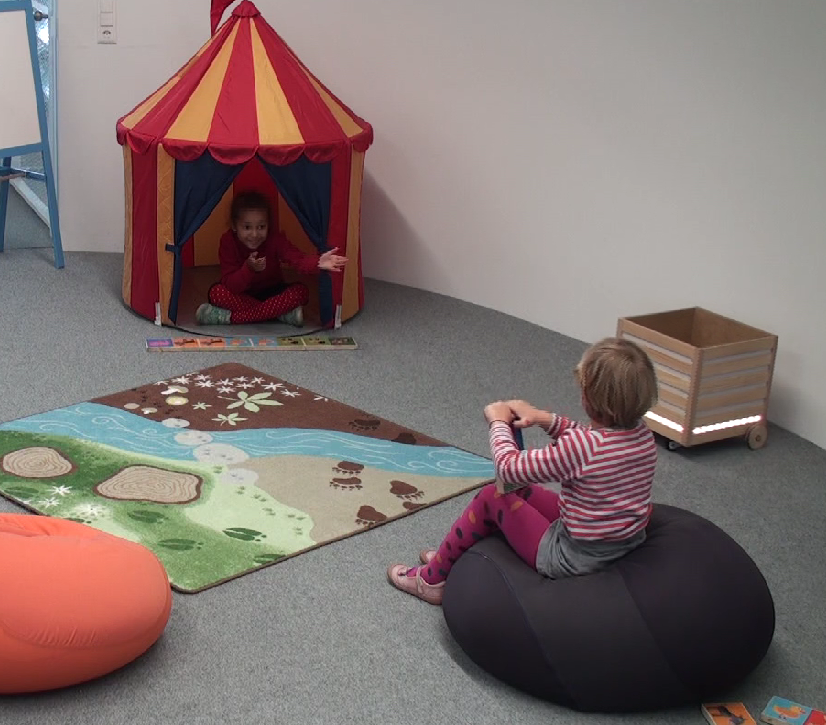
\includegraphics[width=0.6\textwidth]{domino-lost}
    \par
    \only<2>{
        {\bf Hypothesis}: decreased attribution of human-likeness
    }
\end{frame}

\begin{frame}{DISOBEY condition}
    \centering
    Induce the perception of a robot's {\bf own will}
    \par
    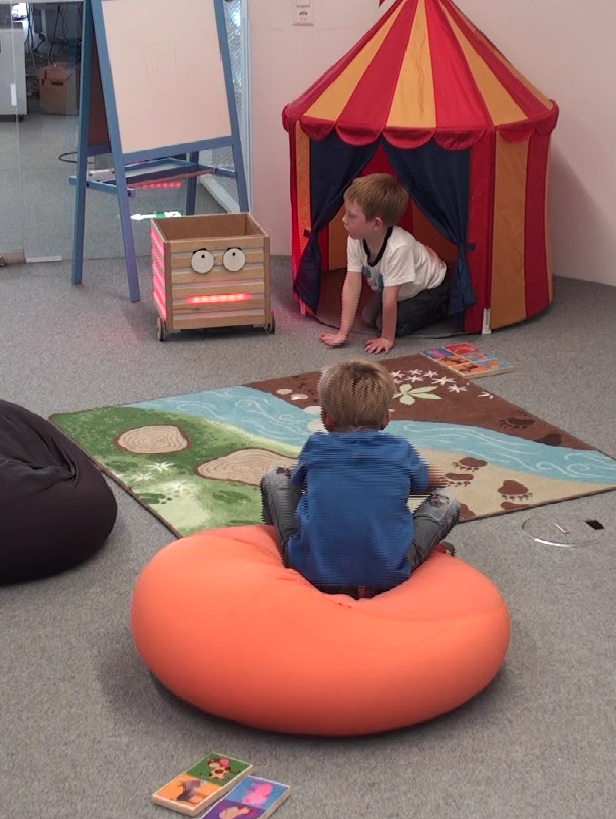
\includegraphics[width=0.5\textheight]{domino-disobey}
    \par
    \only<2>{
        {\bf Hypothesis}: increased attribution of human-likeness
    }
\end{frame}

\begin{frame}{MISTAKE condition}
    \centering
    The robot goes wrong, but recognizes the error and repairs.\\
    {\bf To err is human}! The robot is aware of its own state (introspection)
    and of the expected state of interaction.
    \par
    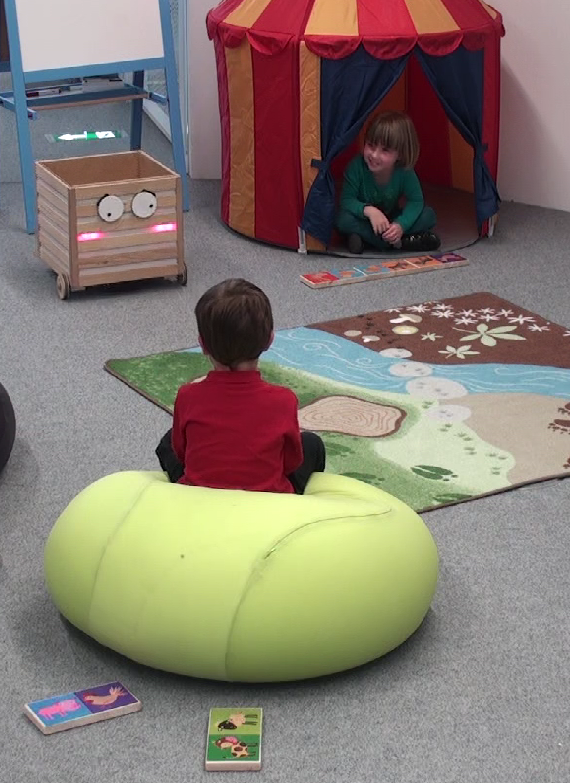
\includegraphics[width=0.5\textheight]{domino-mistake}
    \par
    \only<2>{
        {\bf Hypothesis}: decreased attribution of human-likeness
    }
\end{frame}



\imageframe{domino-mistake}

\begin{frame}{Technical Challenges}
    \begin{itemize}
        \item<1-> Get a child-proof robot to write...
        \item<2-> ...badly...
        \item<3-> Make it able to learn...
        \item<4-> ...with the help of children
    \end{itemize}
\end{frame}

% teaching by learning
\imageframe{domino-setup}

% synchronized writing on a tablet

% generating bad letters
\begin{frame}{Generating Bad Letters}
    \centering
    \only<1> {
    Insight: PCA on a database of hand-written letters to extract characteristic features
    \video{0.8\textwidth}{videos/lost.mp4?start=152&stop=165}
    }

    \only<2> {
    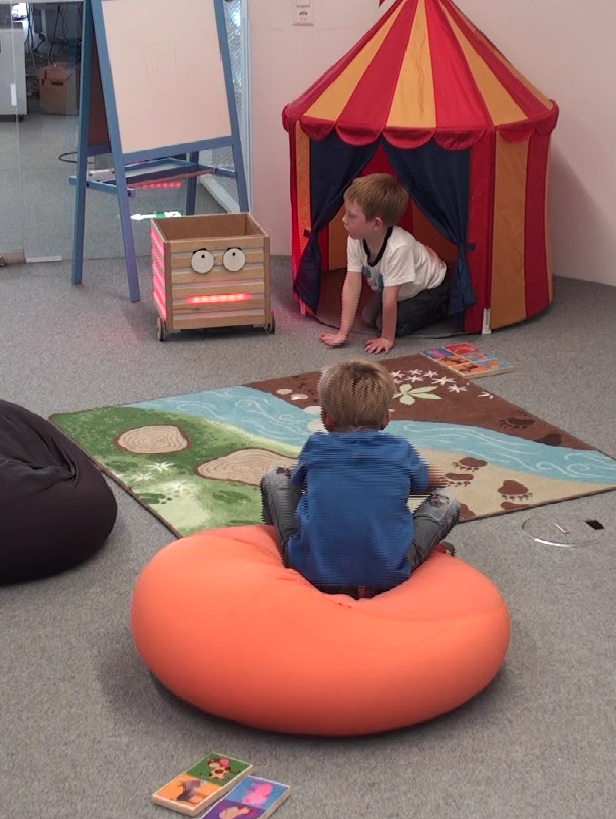
\includegraphics[width=0.8\textwidth]{domino-disobey}
    }
    \only<3> {
    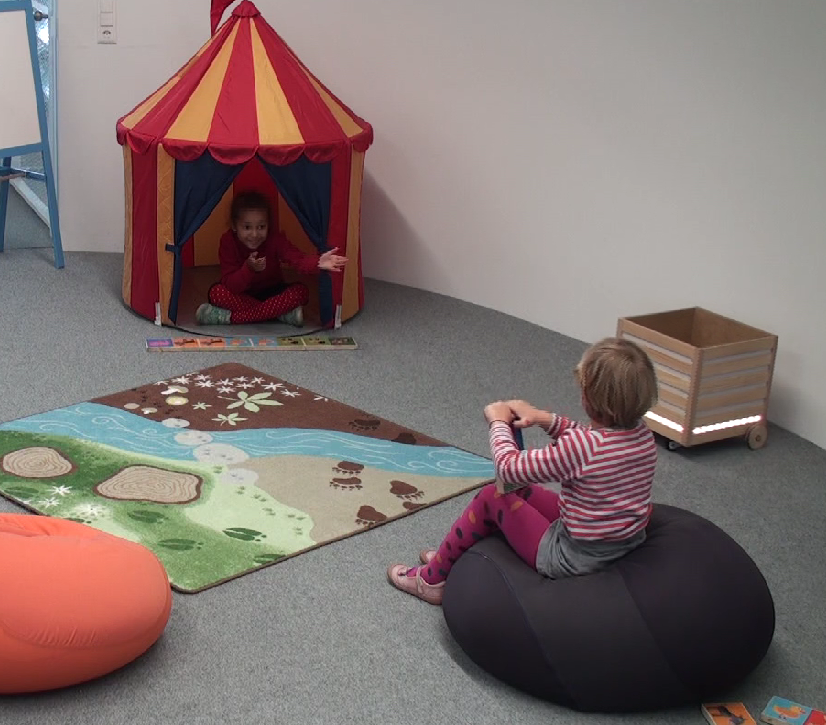
\includegraphics[width=0.6\textwidth]{domino-lost}
    }
\end{frame}

% learning

\begin{frame}{Learning from demonstration}
    \centering
    \only<1> {
    \video{0.8\textwidth}{videos/mistake.mp4?start=184&stop=199}
    }

    \only<2> {
    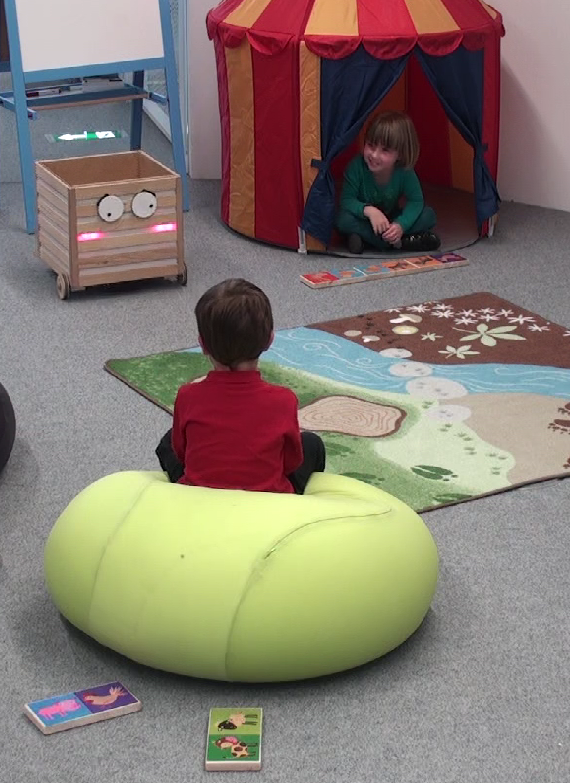
\includegraphics[width=0.8\textwidth]{domino-mistake}
    }
\end{frame}


\begin{frame}{}

\resizebox{0.9\linewidth}{!}{%

\begin{tikzpicture}[
    >=latex,
    node distance=2cm,
    every edge/.style={draw, very thick},
    redarrow/.style={fill=hriSec3, draw=hriSec3},
    greenarrow/.style={fill=hriSec2Dark, draw=hriSec2Dark},
    yellowarrow/.style={fill=hriSec3Comp, draw=hriSec3Comp},
    cmpt/.style={draw, align=center, rounded corners, inner sep=5pt, font=\sf, fill=black!20},
    label/.style={midway, align=left, font=\scriptsize\sf, fill=white, above,opacity=0,text opacity=1}]

    \node at (0,0)[cmpt, fill=hriSec1CompDark!50] (tactile) {tactile interaction \\ manager};
    \node[cmpt, fill=hriSec1CompDark!50, left=of tactile] (display) {display \\ manager};
  
    \node [cmpt, fill=hriSec2Dark!50, below=of tactile] (shape) {shape position \\ manager};
    \node [cmpt, fill=hriSec2Dark!50, left=of shape] (learner) {letter \\ learner};
    \node [cmpt, fill=hriSec2Dark!50, left=of learner] (card) {card \\ detector};

    \node [cmpt, fill=hriSec3Comp!50, below=1.5cm of shape] (writer) {nao writer};
    \node [cmpt, fill=hriSec3Comp!50, left=of writer] (tablet) {tablet detector};
    \node [cmpt, fill=hriSec3Comp!50, left=of tablet] (camera) {nao camera};
    \node [cmpt, fill=hriSec3Comp!50, below=1cm of tablet] (pose) {robot state publisher};

    %%% Relations between components
    \path (tactile) edge [->] node[label] {clear \\ screen} (display);

    \path ($(shape.north west)!0.33!(shape.north east)$) edge [<-] node[label,left] {clear \\ screen} ($(tactile.south west)!0.33!(tactile.south east)$);
    \path ($(shape.north west)!0.66!(shape.north east)$) edge [<-, greenarrow] node[label,right] {feedback \\ + location} ($(tactile.south west)!0.66!(tactile.south east)$);

    \path (shape) edge [->, redarrow] node[label, left, align=right] {letter to write \\ + time \\ + position} (display);
    \path (shape) edge [->,redarrow] node[label, right] {letter to write \\ + time \\ + position in\\tablet frame} (writer);

    \path ($(shape.north west)!0.66!(shape.south west)$) edge [->, greenarrow] node[label,below] {feedback \\ + letter} ($(learner.north east)!0.66!(learner.south east)$);
    \path ($(shape.north west)!0.33!(shape.south west)$) edge [<-, redarrow] node[label] {letter to write \\ + time} ($(learner.north east)!0.33!(learner.south east)$);

    \path (card) edge [->, yellowarrow] node[label] {word to learn} (learner);
    \path (camera) edge [->, yellowarrow] node[label, right] {camera image} (card);
    \path (camera) edge [->, redarrow] node[label] {camera image} (tablet);
    \path (tablet) edge [->, redarrow] node[label] {tablet pose} (writer);
    \path (pose) edge [->, redarrow] node[label, right] {head pose} (tablet);

    \path (-8, 0) edge [->, redarrow] node[label] {Writing letters} (-7, 0);
    \path (-8, -0.6) edge [->, greenarrow] node[label] {Responding to feedback} (-7, -0.6);
    \path (-8, -1.2) edge [->, yellowarrow] node[label] {Detecting card input} (-7, -1.2);
    
\end{tikzpicture}
}

\end{frame}

\section{On the field}

% videos of children
\begin{frame}
    \centering
    \only<1>{
        \video{0.8\textwidth}{videos/lost.mp4}
    }
    \only<2> {
    \video{0.8\textwidth}{videos/lost.mp4}
    }

\end{frame}

\section{A new role?}
\begin{frame}{A new role?}
    \begin{itemize}
        \item<1-> Not a 'tool to teach robotics', not a facilitator
        \item<2-> The robot as 'cognitive agent' is key here (Protégé effect,
            metacognition)
        \item<3-> Could we replace it by someone else? Not easily
    \end{itemize}
\end{frame}

\section{Take home message?}
\begin{frame}{Unexpected behaviours}
    \begin{tabular}{  >{\centering\arraybackslash}m{2cm} | >{\centering\arraybackslash}m{2cm} | >{\centering\arraybackslash}m{2cm} }
        & Unplanned by the robot & Planned by the robot \\ \hline
        Perceived as non-intentional & A  & B  \\ \hline
        Perceived as intentional &  C & D 
    \end{tabular}

\end{frame}

{
\fullbackground{ranger-background.jpg}
\begin{frame}{Anthropomorphism != Engagement}

\begin{figure}
    \hspace*{5cm}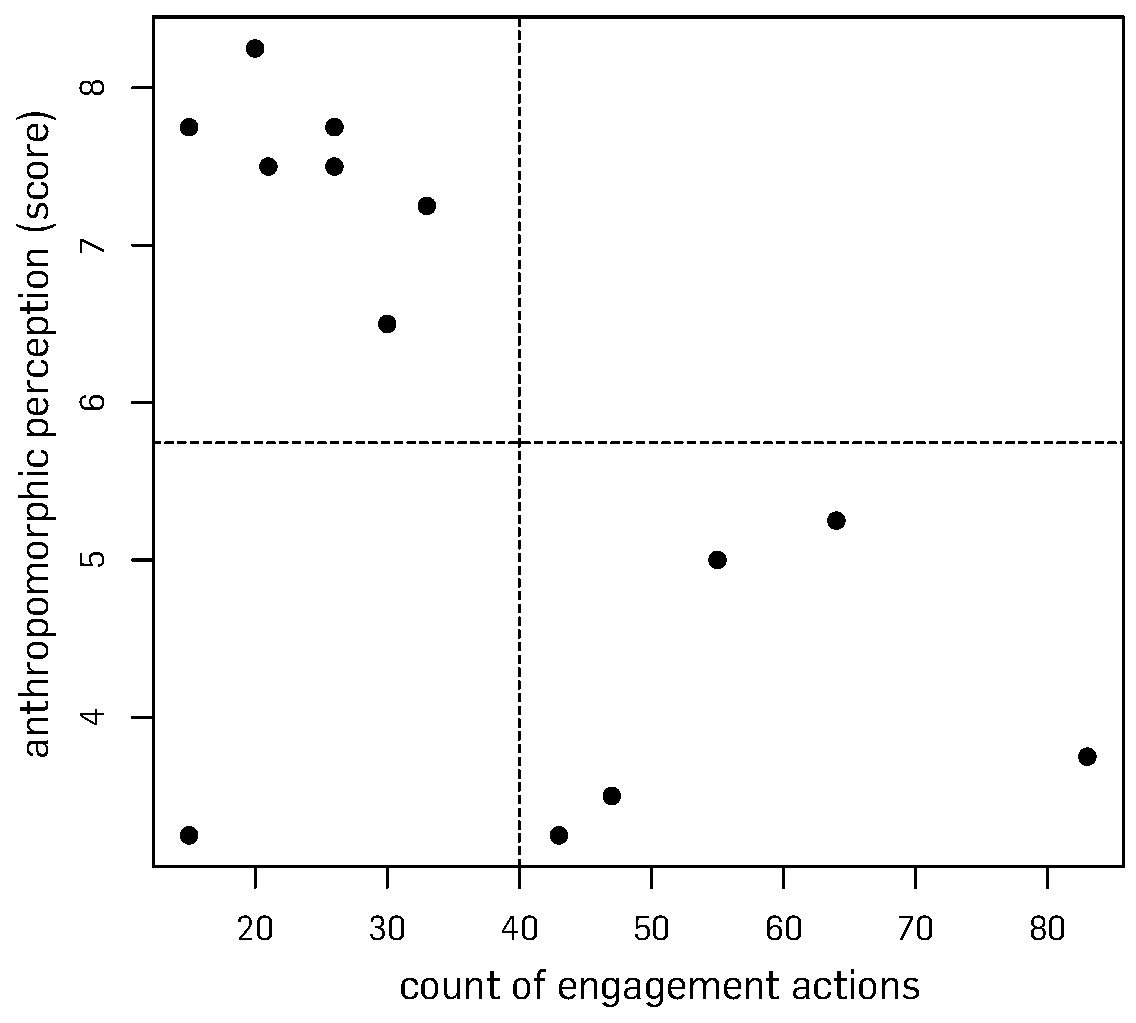
\includegraphics[width=0.6\textwidth]{domino-correlation}
\end{figure}
\end{frame}
}



{
\fullbackground{cheeky-ranger}
\begin{frame}[plain]

\setbeamercolor{hriSec1Demo}{fg=white}
\begin{beamercolorbox}[wd=\linewidth,ht=6ex,dp=0.7ex]{hriSec1Demo}
    \textbf{Thank you!}\\
    \scriptsize
    {\tt alexis.jacq@epfl.ch}\\
    {\tt severin.lemaignan@plymouth.ac.uk}
\end{beamercolorbox}
    \vfill

\end{frame}
}


\end{document}






